\section{Performance}
\label{Section:Performance}

In this section, we provide emperical evidence that supports our claim that, compared to full vectorisation in combination with array fusion, additionally applying vectorisation avoidance results in a net improvement in both compile time and runtime. Our emperical investigation is restricted to the implementation of vectorisation in GHC (as this is to our knowledge the only existing implementation of higher-order flattening) and to targeting multicore CPUs without considering SIMD vector instructions. The results may be different for vector hardware, such as SIMD instructions or GPUs, but currently we have no DPH backend to investigate these architectures.

All benchmarks have been executed on a quadcore 3.4 GHz Intel Core i7 running OS X with the current development version of GHC (version 7.5). With the execption of the benchmarks concerned with load balancing, vectorisation avoidance ought to improve program performance independent of whether the program is executed sequentially or in parallel on multiple cores. We include parallel runtimes thoughout, to support that claim, but only for up to four cores as there are no interesting scalability questions.

\subsection{Additional lambdas}

The encapsulation of maximal sequential subexpressions in lambda abstractions by vectorisation avoidance arguably complicates the program. Does this introduces overheads? In our benchmarks it didn't appear to.

This is not surprising. These lambda abstraction are processed twice by vectorisation: to produce a scalar and a lifted version of the abstraction when creating a vectorised closure (c.f., Section~\ref{sec:vect-closures}). In the case of the lifted code, the lifting transformation \(\LT\cdot\cdot\) introduces additional abstractions anyway. 

In the scalar code, the situation is less obvious. Encapsulation introduces an expression of the form
%
\begin{quote}\small
\begin{alltt}
(\(\lambda\)x\sub{1} \ldots x\sub{n}. expr) x\sub{1} \ldots x\sub{n}
\end{alltt}
\end{quote}
%
This turns into \texttt{Clo\{\ldots\} \capp\ x\sub{1} \capp\ $\cdots$ \capp\ x\sub{n}}, which GHC's simplifier reliably simplified by inlining \texttt{(\capp)}, case simplification, and beta reduction in our experiments. 

\subsection{Simple arithmetic operations}
\label{sec:simple-arith}

\begin{figure*}
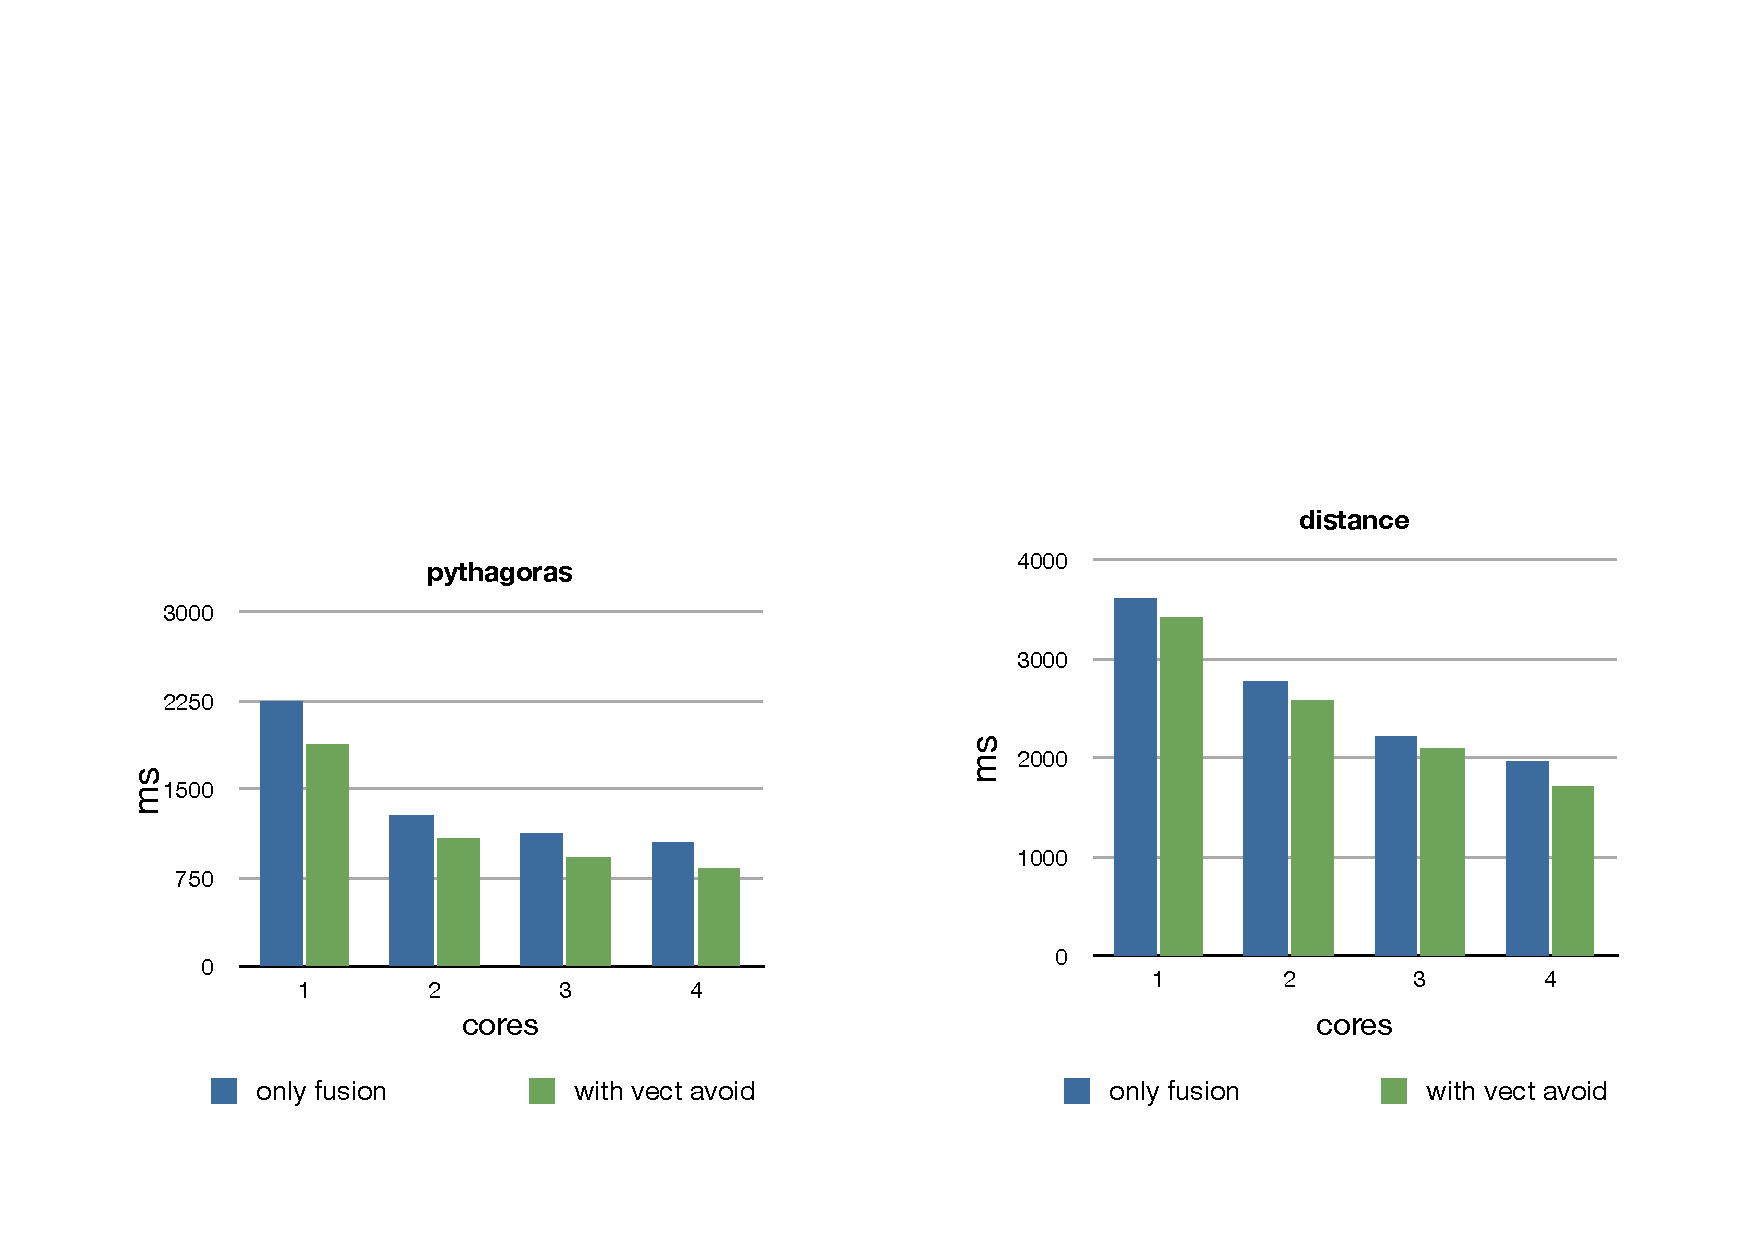
\includegraphics[scale=0.6, trim=0cm 2cm 0cm 8cm, clip]{data/DistancePythagoras.pdf}
\caption{Runtimes of the \texttt{pythagoras} and \texttt{distance} functions on vectors of $10^8$ floating-point numbers}
\label{Figure:distancePythagoras}
\end{figure*}
%
Our first two benchmark programs investigate the case where stream fusion~\cite{coutts:rewriting-strings, coutts:stream-fusion} is able to complete fuse a chain of array traversals. Specifically, we measure the running time of the following two functions when used in parallel --- that is, we measure @zipWith pythagoras xs ys@ and @zipWith distance xs ys@, where @xs@ and @ys@ are vectors containing $10^8$ @Double@ values:
%
\begin{quote}\small
\begin{alltt}
pythagoras x y
  = sqrt (x * x + y * y + 2 * x * y)

distance (xo, yo) ((x1, y1), (x2, y2))
  = (x1 - xo) * (y2 - yo) - (y1 - yo) * (x2 - xo)
\end{alltt}
\end{quote}
%
In our current implementation, the @Scalar@ class does not yet have an instance for pairs. Hence, vectorisation avoidance cannot use @zipWith_scalar@ on the entire body of @distance@. Instead it encapsulates the body of
the innermost case expression (performing pattern matching on the pairs); so, the code has the following structure after encapsulation:
%
\begin{quote}\small
\begin{alltt}
distance xy0 xy =
 case xy0 of (x0, y0) -> 
  case xy of (xy1, xy2) -> 
   case xy1 of (x1, y1) ->
    case xy2 of (x2, y2) -> 
     (\(\lambda\) x0 y0 x1 y1 x2 y2. 
       (x1 - x0) * (y2 - y0) - (y1 - y0) * (x2 - x0)) 
     x0 y0 x1 y1 x2 y2
\end{alltt}
\end{quote}
%
Given that the additional array traversals introduced by vectorisation of @pythagoras@ and @distance@ can be completely eliminated by array fusion, we might expect that vectorisation avoidance does not provide any additional benefit. However, the graph displayed in Figure~\ref{Figure:distancePythagoras} shows that vectorisation avoidance does improve performance slightly. This is as fusion results in slightly more complex loops than vectorisation avoidance.

According to the graph, the two benchmarks don't scale particularily well. In our opinion, this is as the code is memory bound --- i.e., the full floating-point performance of the processor is not exploited as the processor has to wait for the memory-subsystem to fetch the operands.

\subsection{Fusion and vectorisation avoidance together}

\begin{figure*}
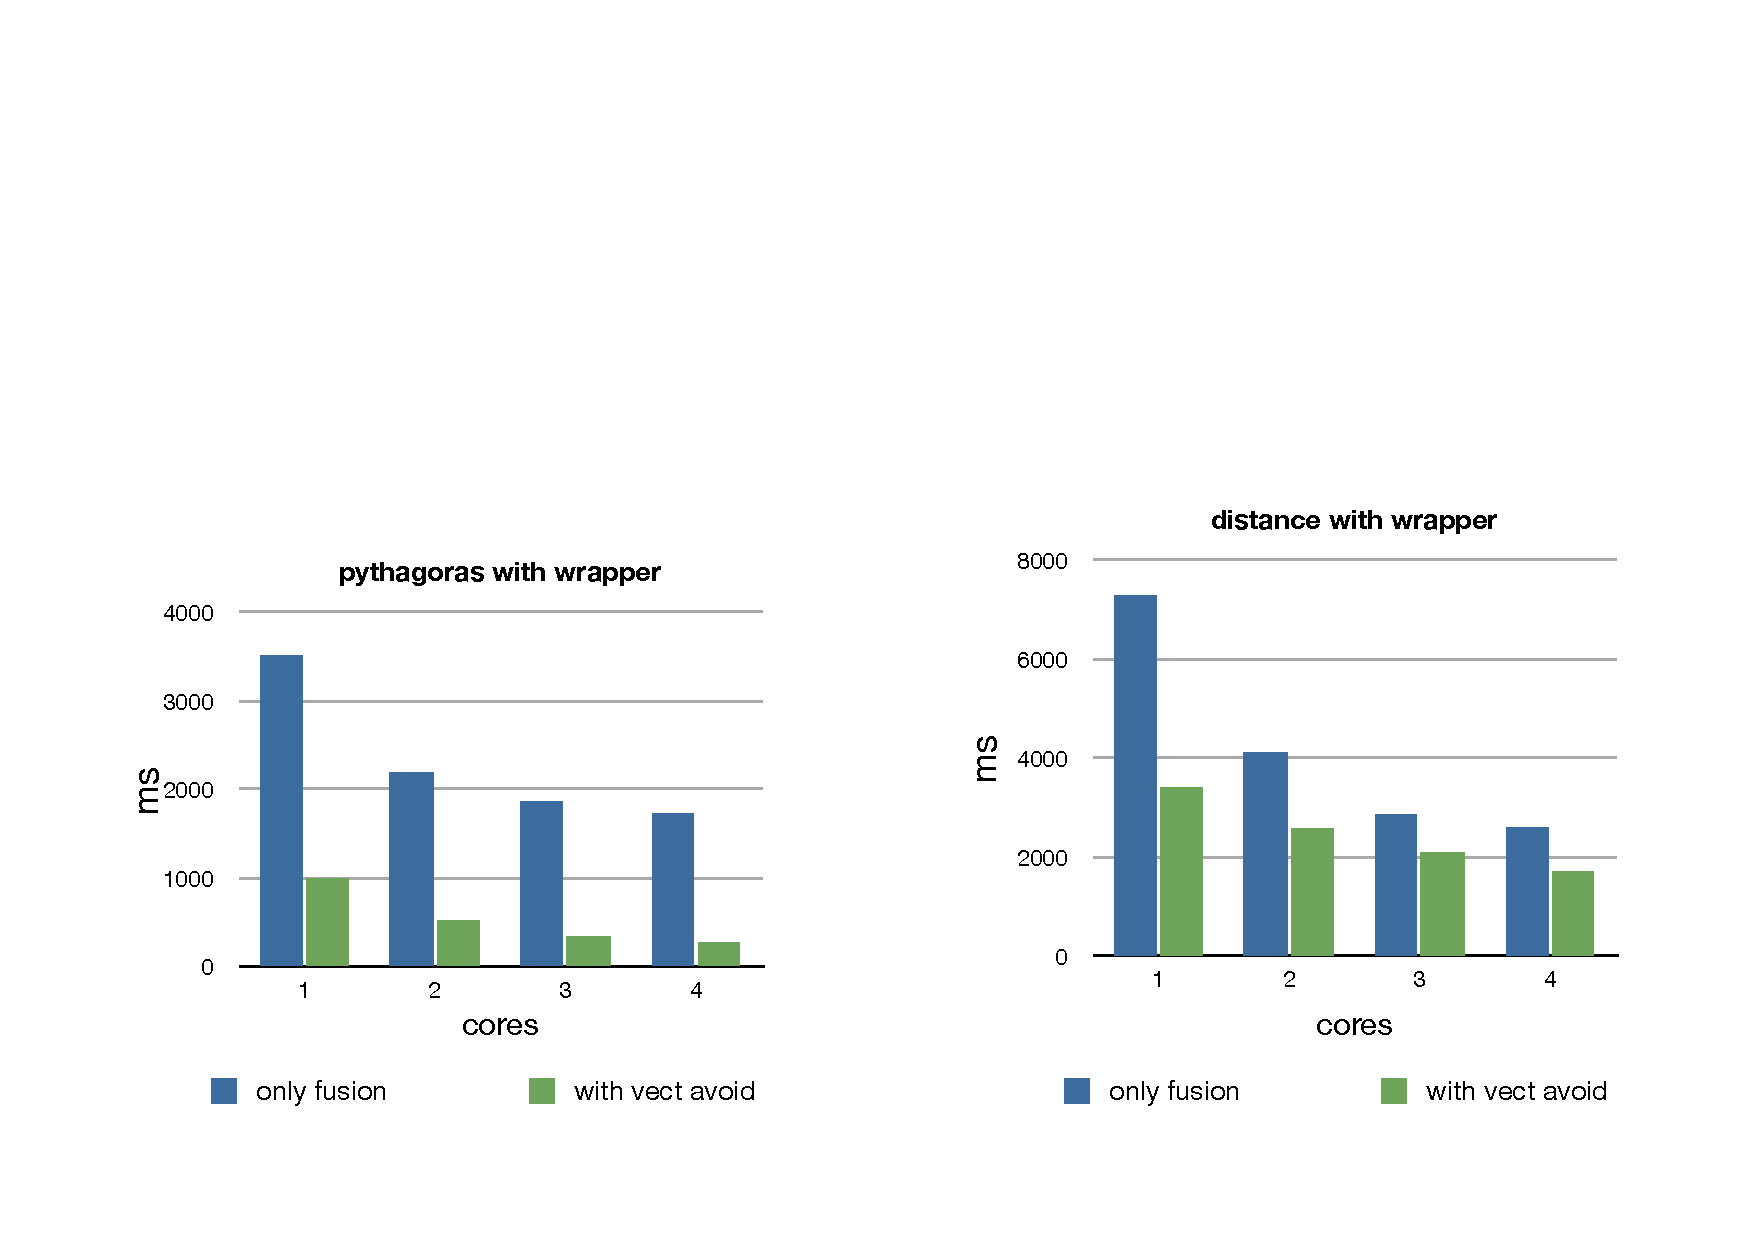
\includegraphics[scale=0.6, trim=0cm 2cm 0cm 8cm, clip]{data/DistPythagorasInl.pdf}
\caption{Runtimes of the \texttt{pythagoras} and \texttt{distance} functions \emph{with wrappers} on vectors of $10^8$ floating-point numbers}
\label{Figure:distancePythagorasInl}
\end{figure*}
%
In the previous benchmark, we measured the performance of @zipWithP pythagoras xs ys@ by itself (and the same with @distance@). Next, we have a look at that same code sandwiched between a producer (enumerating the arrays consumed by the @zipWithP@) and a consumer (summing up the result array with @sumP@); so, we have got
%
\begin{quote}\small
\begin{code}
sumP (zipWithP pythagoras 
               (enumFromToP 1 (10^8)) 
               (enumFromToP 1 (10^8)))
\end{code}
\end{quote}
%
Ideally, we would like the whole pipeline to fuse into a single loop that computes the final sum without creating any intermediate arrays. Looking at the graph in Figure~\ref{Figure:distancePythagorasInl} that does happen for the @pythagoras@ benchmark with vectorisation avoidance enabled. However, with fusion alone, performance is worse by more than a factor of 3. Array fusion by itself did not manage to eliminate the entire pipeline, whereas the combination of array fusion with vectorisation avoidance did that successfully leading to a dramatic performance improvement. Once the pipeline fuses completely, the code also scales better --- as there are no more intermediate structures, the memory-access bottleneck vanishes.

Why is fusion by itself not successful at removing all intermediate structures? In the lifted code, the arrays produced by the enumerations are shared, as the arguments to @pythagoras@ are used multiple times in the body. This hampers inlining, and hence, stream fusion. With vectorisation avoidance, all sharing is in the code that isn't vectorised, so this problem does not arise.

In the case of @distance@, vectorisation avoidance is also a clear improvement. However, it is less dramatic as the remaining pattern matching of the argument pairs (discussed in the previous subsection) prevents fusion of the entire pipeline.

\subsection{Conditionals}

\begin{figure*}
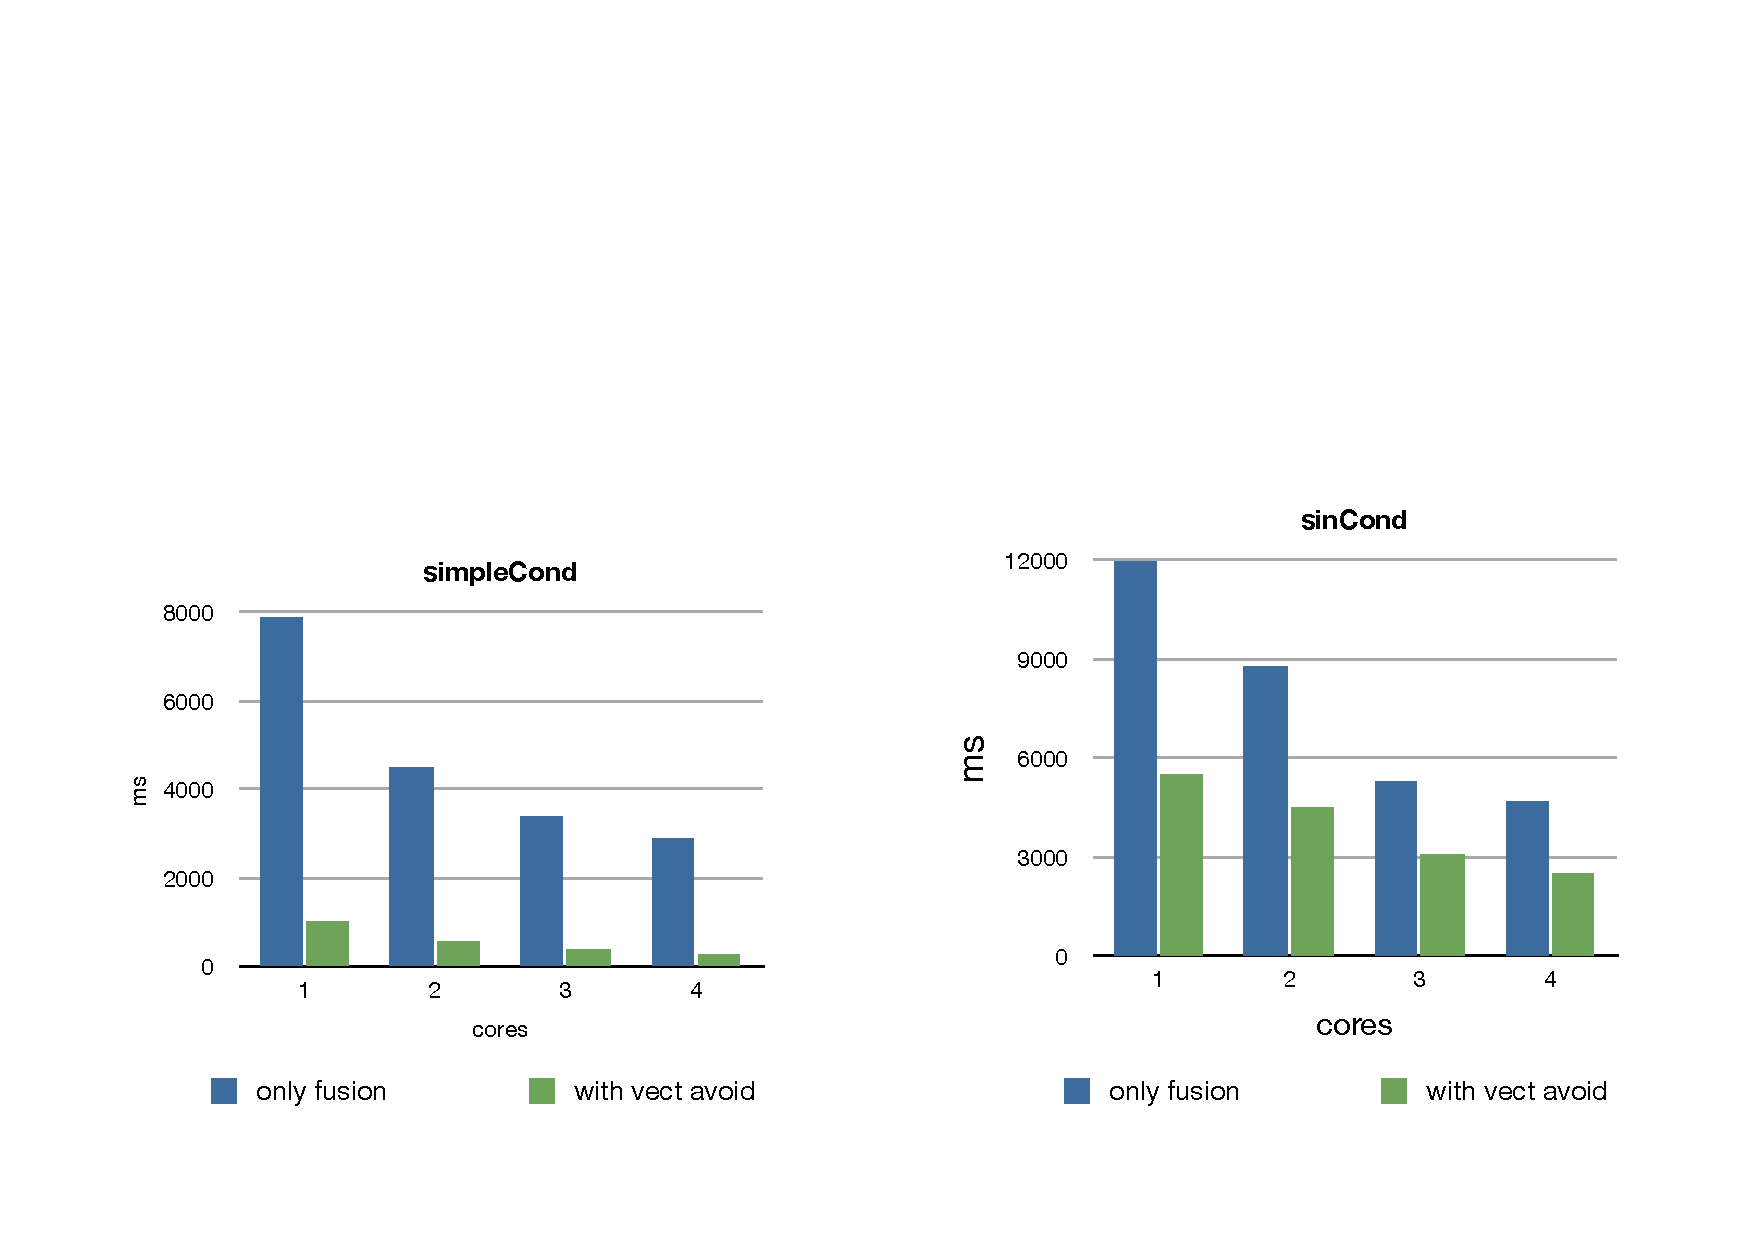
\includegraphics[scale=0.6, trim=0cm 2cm 0cm 8cm, clip]{data/Conditional.pdf}
\caption{Runtimes of the \texttt{simpleCond} and \texttt{sinCond} functions on vectors of $10^8$ \texttt{Int}s and \texttt{Double}s, respectively}
\label{Figure:Conditional}
\end{figure*}
%
Fully vectorising conditionals is expensive due to the @spliPA@ and @combinePA@ operations. On the other hand, vectorised conditionals balance load very well, whereas if vectorisation is avoided, we might suffer from load imbalance. To assess the impact of vectorisation avoidance on conditionals, we measured @mapP simpleCond xs@ and @mapP sinCond xs@, for arrays with $10^8$ elements, where
%
\begin{quote}\small
\begin{alltt}
simpleCond x = if (x `mod` 2 == 0) 
               then 3 * x 
               else 2 * x

sinCond n = if (x < n / 2) 
            then  x 
            else sin (sin (sin (2 * x)))
\end{alltt}
\end{quote}
%
We chose the input array to contain the increasing sequence of 1 to the size of the array. Hence, for @simpleCond@, we have no load imbalance with vectorisation avoidance, whereas @sinCond@ has a severe load imbalance as we execute the then-branch on the first half of elements and the else-branch on the other half.

As expected, the graph in Figure~\ref{Figure:Conditional} shows that vectorisation avoidance for conditionals is a big improvement when there is no load imbalance. However, even with a severe load imbalance, vectorisation avoidance is still an advantage for small numbers of cores. Nevertheless, with vectorisation avoidance, scalability suffers in case of load imbalance; hence, it would be worthwhile to enable the programmer to determine the behaviour of the vectoriser with a pragma.

% In the second example, the time necessary for evaluating the two branches differs, and applied to the ordered array we use as input, there is a significant load imbalance, as the alternative is only called on elements of the second half of the array. In practice, we find that this degree of imbalance is fairly rare. As we would expect, the relative speedup for the fully vectorised version is slightly better (2.7) than for the one compiled with vectorisation avoidance (2.2), but in absolute terms, the latter version is, even on four PEs. more the 50\% faster. It may seem surprising that the difference is not bigger. However, redistributing the data involves communication, which in turn is more expensive the more
% PEs are involved, putting a cap on the possible speedup.
% In general, vectorisation avoidance will yield the better results for scalar conditionals with constant work complexity. However, it does not seem reasonable to
% stick with one fixed compilation strategy for the whole program in this case, as it is definitely possible to write programs for which either would be a bad choice. The programmer should have the possibility two enforce a particular strategy via a code pragma. We have not implemented such a pragma yet, but the transformation could be adapted easily to handle this.

\subsection{Recursive Functions}

\begin{figure}
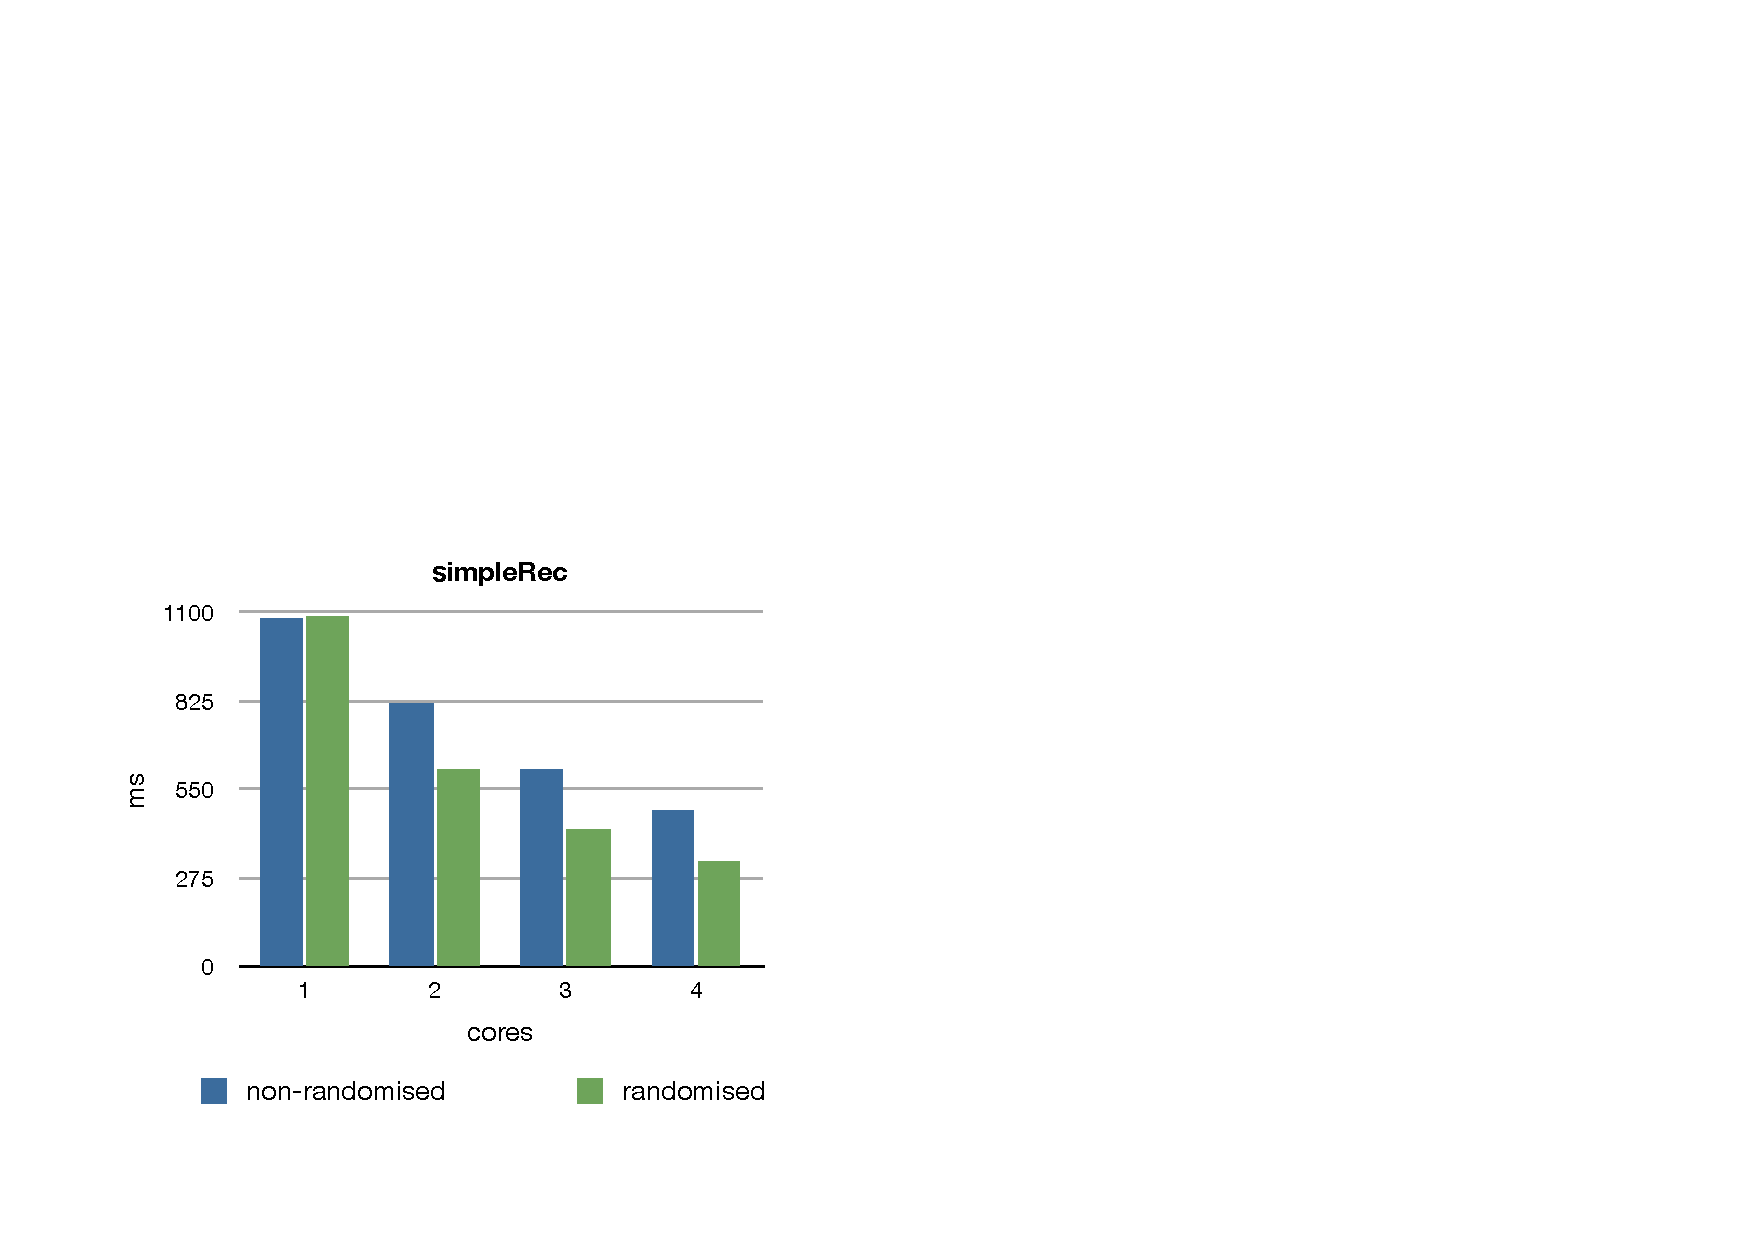
\includegraphics[scale=0.6, trim=0cm 2cm 0cm 9cm, clip]{data/Recursion.pdf}
\caption{Runtimes of \texttt{simpleRec} on vectors of $10^5$ \texttt{Double}s with and without randomisation}
\label{Figure:Recursion}
\end{figure}
%
The question of load imbalance becomes even more pressing when the work complexity of a function depends on the array element it is applied to, as in
%
\begin{quote}\small
\begin{alltt}
simpleRec x = if (x < 5) 
              then x 
              else simpleRec (x - 5)
\end{alltt}
\end{quote}
%
Interestingly, in the case of a tail recursive function, the benefit of vectorisation avoidance is even greater, as vectorisation prevents the code generator compiling the recursion into a simple loop. For the admittedly extreme case of @simpleRec@, where there is no work in the recursive steps, the fully vectorised version is two orders of magnitude slower than when we use vectorisation avoidance.

Unfortunately, when mapping @simpleRec@ over an array containing the increasing sequence of 1 to the size of the array, load imbalance is also significant. Vectorisation of @simpleRec@ provides load balancing, but, in this example, with a prohibitively expensive constant factor. An alternative to full vectorisation in such cases is to apply vectorisation avoidance, but to randomise the input vector. The graph in Figure~\ref{Figure:Recursion} suggests that this is a worthwhile strategy. Currently, a programmer needs to do it explicitly, but we plan to investigate automatic randomisation.

\subsection{Calculating accelerations}

\begin{figure}
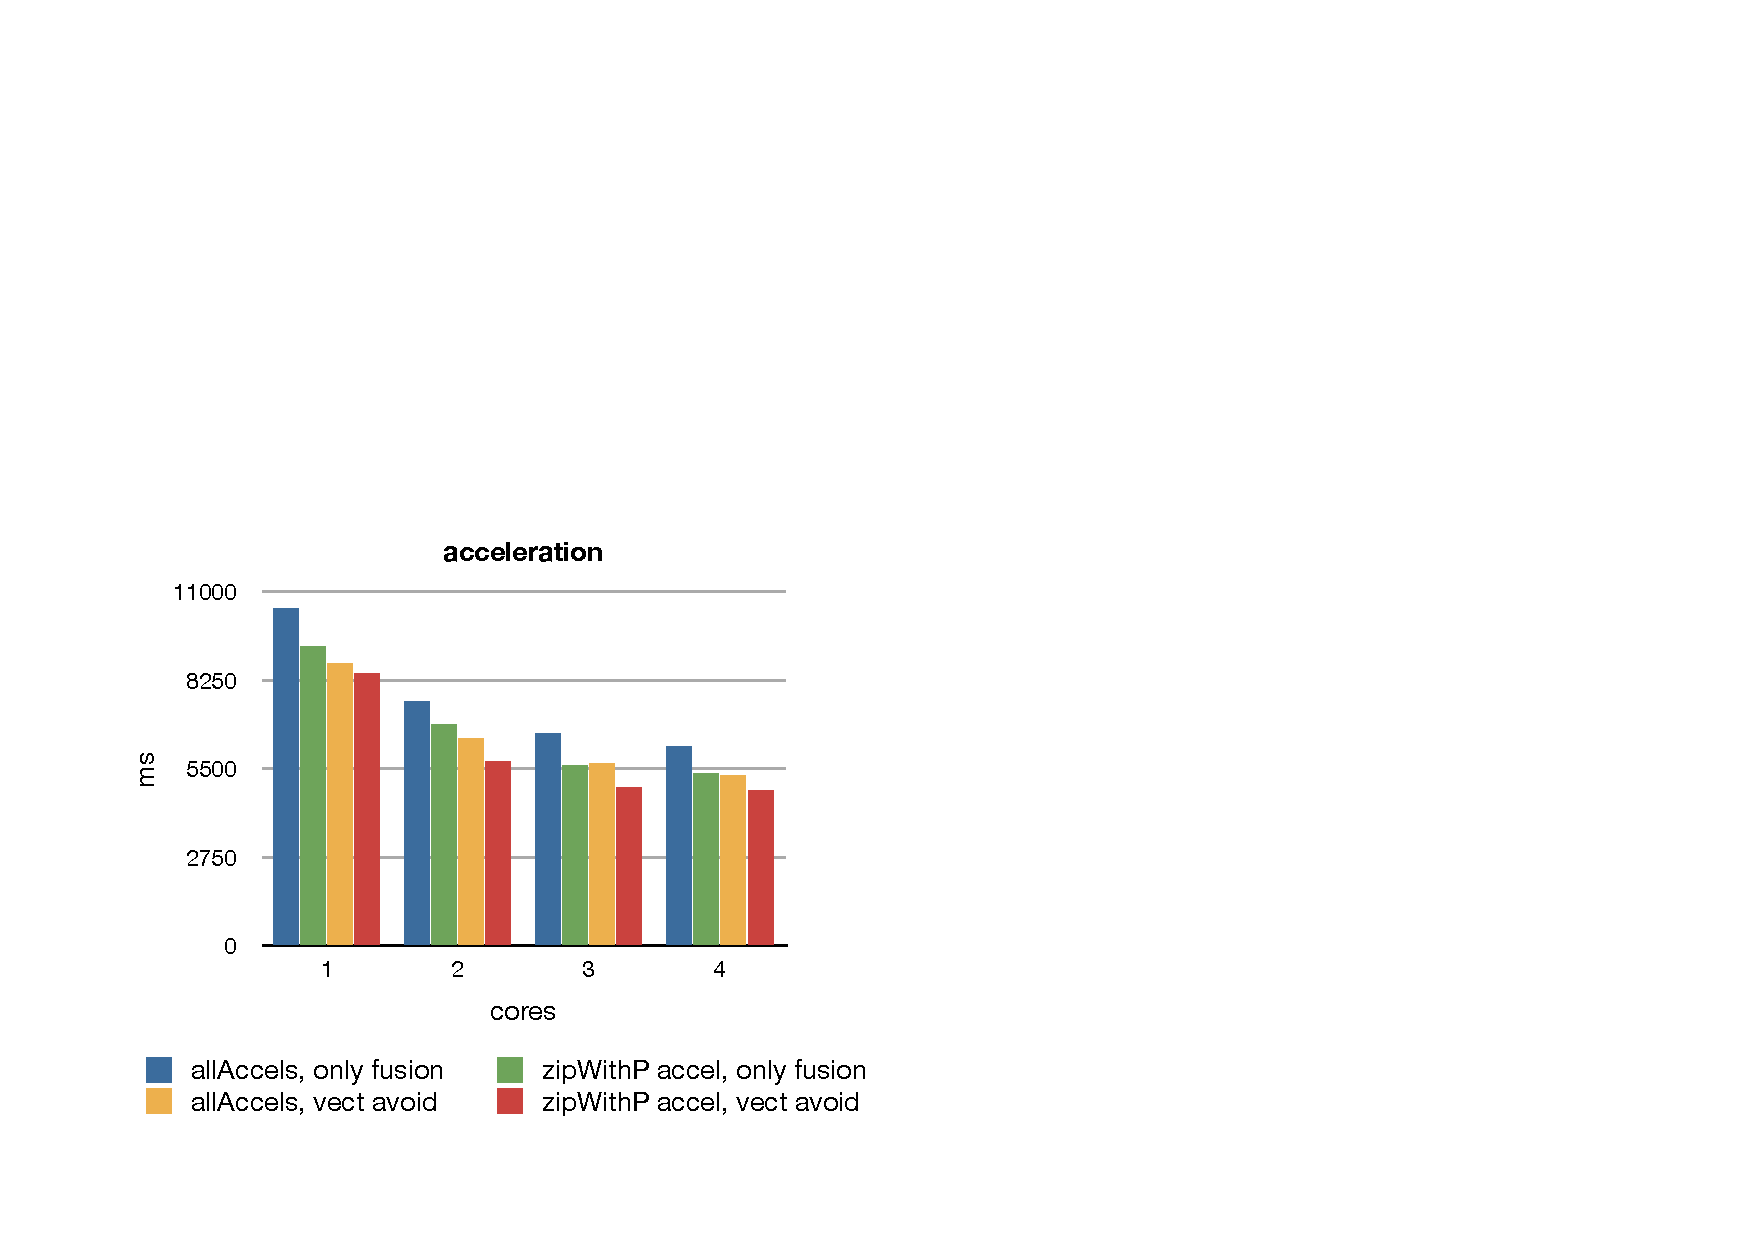
\includegraphics[scale=0.6, trim=1.5cm 2cm 0cm 9cm, clip]{data/Accel.pdf}
\caption{Runtimes of \texttt{allAccels} and \texttt{zipWithP accels} computing $10^8$ interactions}
\label{Figure:Accel}
\end{figure}
%
Figure~\ref{Figure:Accel} displays the running times for computing the acceleration of $10^8$ mass point interactions with and without vectorisation avoidance. It does so in two ways. Firstly, by using @allAccels@ on $10^4$ mass points (it implements a quadratic algorithm); and secondly, by directly using @zipWithP accel@ on two arrays of $10^8$ mass points. The main difference between these two computations is that @allAccels@ also computes $2*10^4$ parallel sums. Hence, it is not surprising that @allAccels@ is slower than @zipWithP accel@ across the board.

However, it is interesting to see that the gain due to vectorisation avoidance is higher in the case of @allAccels@, where it is 11\% on a single core, than for @zipWithP accel@, where it is 3\%. The reason is as for @pythagoras@ and @distance@ with wrappers. Fusion of the acceleration computation with @sumP@ is more effective with vectorisation avoidance.

Note also that, as previously mentioned, the @Scalar@ class in our current implementation does not yet include pairs. Hence, the vectorisation of @accel@ cannot yet be entirely avoided (c.f., the explanation for @distance@ in Section~\ref{sec:simple-arith}). We expect the gain to be even more pronnounced once that is the case.

\subsection{Compilation time}

We argued that, apart from producing faster code, vectorisation avoidance also produces simpler code which requires fewer subsequent optimisations.  This, in turn, should result in shorted compilation times.  For the examples presented in this section, overall compilation was about 25\% faster when vectorisation avoidance was enabled.
